%&tex

\documentclass[usenames,dvipsnames]{beamer}

\usepackage[english]{babel}
\usepackage[utf8]{inputenc}
\usepackage[T1]{fontenc}
\usepackage{csquotes}
\usepackage{mathtools}
\usepackage{amsthm}
\usepackage{amssymb}
\usepackage{thmtools,thm-restate}
\usepackage{amsfonts}
\usepackage{hyperref}
\usepackage[singlelinecheck=false]{caption}
\usepackage[backend=biber,url=true,doi=true,eprint=false,style=authoryear]{biblatex}
\usepackage{algorithm}
\usepackage[noend]{algpseudocode}
\usepackage{listings}
\usepackage{subcaption}
\usepackage{booktabs}
\usepackage{textcomp}
\usepackage{xcolor,colortbl}
\usepackage{multirow}
\usepackage{multicol}
\usepackage{pgfplots}
\usepackage{tikz}
\usetikzlibrary{shapes,arrows,positioning,fit,circuits.logic.US}
\pgfplotsset{compat=1.17}

\usefonttheme[onlymath]{serif}

\def\BibTeX{{\rm B\kern-.05em{\sc i\kern-.025em b}\kern-.08em T\kern-.1667em\lower.7ex\hbox{E}\kern-.125emX}}
\definecolor{Gray}{gray}{0.5}
\definecolor{Cyan}{rgb}{0.9,1,1}
\definecolor{Yellow}{rgb}{0.7,0.98,0.98}

\addbibresource{./references.bib}
\usetheme{boxes}

\AtBeginSection{\frame{\sectionpage}}

\setbeamertemplate{section page}{
  \begin{centering}
  \begin{beamercolorbox}[sep=12pt,center]{part title}
  \usebeamerfont{section title}\insertsection\par
  \end{beamercolorbox}
  \end{centering}
}

\DeclareMathOperator*{\argmin}{arg\,min}
\DeclareMathOperator*{\argmax}{arg\,max}
\DeclareMathOperator*{\Val}{\text{Val}}
\DeclareMathOperator*{\Ch}{\text{Ch}}
\DeclareMathOperator*{\Pa}{\text{Pa}}
\DeclareMathOperator*{\Sc}{\text{Sc}}
\newcommand{\ov}{\overline}
\newcommand{\tsup}{\textsuperscript}

\newcommand\defeq{\mathrel{\overset{\makebox[0pt]{\mbox{\normalfont\tiny\sffamily def}}}{=}}}

\newcommand{\algorithmautorefname}{Algorithm}
\algrenewcommand\algorithmicrequire{\textbf{Input}}
\algrenewcommand\algorithmicensure{\textbf{Output}}
\algnewcommand{\LineComment}[1]{\State\,\(\triangleright\) #1}

\newcommand{\Left}{\text{LEFT}}
\newcommand{\Right}{\text{RIGHT}}
\newcommand{\Up}{\text{UP}}

\newcommand{\set}[1]{\mathbf{#1}}
\newcommand{\pr}{\text{P}}
\newcommand{\eps}{\varepsilon}
\newcommand{\ddspn}[2]{\frac{\partial#1}{\partial#2}}
\newcommand{\iddspn}[2]{\partial#1/\partial#2}
\newcommand{\indep}{\perp}
\renewcommand{\implies}{\Rightarrow}

\newcommand{\bigo}{\mathcal{O}}
\newcommand{\mbf}[1]{\mathbf{#1}}

\setbeamertemplate{theorems}[ams style]

\setbeamersize{description width=1.0cm}

\lstset{frameround=fttt,
	numbers=left,
	breaklines=true,
	keywordstyle=\bfseries,
	basicstyle=\ttfamily,
}

\newcommand{\code}[1]{\lstinline[mathescape=true]{#1}}
\newcommand{\mcode}[1]{\lstinline[mathescape]!#1!}

\newcommand\blfootnote[1]{%
  \begingroup
  \renewcommand\thefootnote{}\footnote{#1}%
  \addtocounter{footnote}{-1}%
  \endgroup
}

\DeclareMathOperator{\Sum}{\normalfont{S}}
\DeclareMathOperator{\Sums}{\mathbf{S}}
\DeclareMathOperator{\Prod}{\normalfont{P}}
\DeclareMathOperator{\Prods}{\mathbf{P}}
\DeclareMathOperator{\Leaf}{\normalfont{L}}
\DeclareMathOperator{\Leaves}{\mathbf{L}}
\DeclareMathOperator{\Node}{\normalfont{N}}
\DeclareMathOperator{\Nodes}{\mathbf{N}}
\DeclareMathOperator{\Child}{\normalfont{C}}
\DeclareMathOperator{\Children}{\mathbf{C}}
\DeclareMathOperator{\Conj}{\otimes}
\DeclareMathOperator{\Disj}{\oplus}

\newcommand{\newGraphNode}[4]{\node[#4] (#1) at (#2) {\rotatebox{-90}{#3}}}
\newcommand{\newAndNode}[4]{\node[#4,and gate,fill=blue!50!red!30] (#1) at (#2) {\rotatebox{-90}{#3}}}
\newcommand{\newOrNode}[4]{\node[#4,or gate,fill=blue!50!green!30] (#1) at (#2) {\rotatebox{-90}{#3}}}

\definecolor{palette1}{HTML}{0066ff}
\definecolor{palette2}{HTML}{669900}
\definecolor{palette3}{HTML}{ff3300}

%\newcommand{\full}{}
\newcommand{\iffull}[1]{%
  \ifcsname full\endcsname%
    #1
  \fi
}

\definecolor{LightGray}{gray}{0.85}

\colorlet{tableheadcolor}{gray!25} % Table header colour = 25% gray
\newcommand{\headcol}{\rowcolor{tableheadcolor}} %
\colorlet{tablerowcolor}{gray!10} % Table row separator colour = 10% gray
\newcommand{\rowcol}{\rowcolor{tablerowcolor}} %
    % Command \topline consists of a (slightly modified) \toprule followed by a \heavyrule rule of colour tableheadcolor (hence, 2 separate rules)
\newcommand{\topline}{\arrayrulecolor{black}\specialrule{0.1em}{\abovetopsep}{0pt}%
            \arrayrulecolor{tableheadcolor}\specialrule{\belowrulesep}{0pt}{0pt}%
            \arrayrulecolor{black}}
    % Command \midline consists of 3 rules (top colour tableheadcolor, middle colour black, bottom colour white)
\newcommand{\midline}{\arrayrulecolor{tableheadcolor}\specialrule{\aboverulesep}{0pt}{0pt}%
            \arrayrulecolor{black}\specialrule{\lightrulewidth}{0pt}{0pt}%
            \arrayrulecolor{white}\specialrule{\belowrulesep}{0pt}{0pt}%
            \arrayrulecolor{black}}
    % Command \rowmidlinecw consists of 3 rules (top colour tablerowcolor, middle colour black, bottom colour white)
\newcommand{\rowmidlinecw}{\arrayrulecolor{tablerowcolor}\specialrule{\aboverulesep}{0pt}{0pt}%
            \arrayrulecolor{black}\specialrule{\lightrulewidth}{0pt}{0pt}%
            \arrayrulecolor{white}\specialrule{\belowrulesep}{0pt}{0pt}%
            \arrayrulecolor{black}}
    % Command \rowmidlinewc consists of 3 rules (top colour white, middle colour black, bottom colour tablerowcolor)
\newcommand{\rowmidlinewc}{\arrayrulecolor{white}\specialrule{\aboverulesep}{0pt}{0pt}%
            \arrayrulecolor{black}\specialrule{\lightrulewidth}{0pt}{0pt}%
            \arrayrulecolor{tablerowcolor}\specialrule{\belowrulesep}{0pt}{0pt}%
            \arrayrulecolor{black}}
    % Command \rowmidlinew consists of 1 white rule
\newcommand{\rowmidlinew}{\arrayrulecolor{white}\specialrule{\aboverulesep}{0pt}{0pt}%
            \arrayrulecolor{black}}
    % Command \rowmidlinec consists of 1 tablerowcolor rule
\newcommand{\rowmidlinec}{\arrayrulecolor{tablerowcolor}\specialrule{\aboverulesep}{0pt}{0pt}%
            \arrayrulecolor{black}}
    % Command \bottomline consists of 2 rules (top colour
\newcommand{\bottomline}{\arrayrulecolor{white}\specialrule{\aboverulesep}{0pt}{0pt}%
            \arrayrulecolor{black}\specialrule{\heavyrulewidth}{0pt}{\belowbottomsep}}%
\newcommand{\bottomlinec}{\arrayrulecolor{tablerowcolor}\specialrule{\aboverulesep}{0pt}{0pt}%
            \arrayrulecolor{black}\specialrule{\heavyrulewidth}{0pt}{\belowbottomsep}}%

\input{led}

\title{Learning Probabilistic Sentential Decision Diagrams by Sampling}
\subtitle{~\\KDMiLe 2020}
\date{}
\author[R. L. Geh, D. D. Mauá, A. Antonucci]{\textbf{Renato Geh}\inst{1} \and Denis Mauá\inst{1}
  \and Alessandro Antonucci\inst{2}}
\institute[USP, IDSIA]{\inst{1} Institute of Mathematics and Statistics, University of São Paulo,
  Brazil\\\texttt{\{renatolg,ddm\}@ime.usp.br} \and \inst{2} Istituto Dalle Molle di Studi
sull'Intelligenza Artificiale, Switzerland\\\texttt{alessandro@idsia.ch}}

\begin{document}

\maketitle

%\section{Motivation}

%\begin{frame}
  %\frametitle{Why Probabilistic Sentential Decision Diagrams?}

  %\begin{align*}
    %\text{\textbf{Observable segments:}}\quad &\set{Y}=\{Y_1,Y_2,\ldots,Y_7\}\\
    %\text{\textbf{Latent segments:}}\quad &\set{X}=\{X_1,X_2,\ldots,X_7\}
  %\end{align*}

  %\begin{center}
    %\sevensegnum[size=1.5em,line width=0.2em]{4}\\\small
    %$\phi_4 = \neg X_1 \wedge  X_2 \wedge  X_3 \wedge \neg X_4 \wedge \neg X_5 \wedge  X_6 \wedge  X_7$
  %\end{center}
  %\begin{center}
    %\sevensegnum[size=1.5em,line width=0.2em]{7}\\\small
    %$\phi_7 =  X_1 \wedge  X_2 \wedge  X_3 \wedge \neg X_4 \wedge \neg X_5 \wedge \neg X_6 \wedge \neg X_7$
  %\end{center}

  %\begin{center}
    %\parbox{0.8\textwidth}{
      %Given $\set{Y}=\set{y}$, find
      %\begin{equation*}
	%\hat{\set{x}}=\argmax_{\set{x}} p(\set{x}|\set{y}),
      %\end{equation*}
      %such that $\hat{\set{x}}$ is a valid digit following a formula $\phi_d$.
    %}
  %\end{center}

  %%0 & $\phi_0 =  X_1 \wedge  X_2 \wedge  X_3 \wedge  X_4 \wedge  X_5 \wedge  X_6 \wedge \neg X_7$\\
  %%1 & $\phi_0 = \neg X_1 \wedge  X_2 \wedge  X_3 \wedge \neg X_4 \wedge \neg X_5 \wedge \neg X_6 \wedge \neg X_7$\\
  %%2 & $\phi_0 =  X_1 \wedge  X_2 \wedge \neg X_3 \wedge  X_4 \wedge  X_5 \wedge \neg X_6 \wedge  X_7$\\
  %%3 & $\phi_0 =  X_1 \wedge  X_2 \wedge  X_3 \wedge  X_4 \wedge \neg X_5 \wedge \neg X_6 \wedge  X_7$\\
  %%4 & $\phi_0 = \neg X_1 \wedge  X_2 \wedge  X_3 \wedge \neg X_4 \wedge \neg X_5 \wedge  X_6 \wedge  X_7$\\
  %%5 & $\phi_0 =  X_1 \wedge \neg X_2 \wedge  X_3 \wedge  X_4 \wedge \neg X_5 \wedge  X_6 \wedge  X_7$\\
  %%6 & $\phi_0 =  X_1 \wedge \neg X_2 \wedge  X_3 \wedge  X_4 \wedge  X_5 \wedge  X_6 \wedge  X_7$\\
  %%7 & $\phi_0 =  X_1 \wedge  X_2 \wedge  X_3 \wedge \neg X_4 \wedge \neg X_5 \wedge \neg X_6 \wedge \neg X_7$\\
  %%8 & $\phi_0 =  X_1 \wedge  X_2 \wedge  X_3 \wedge  X_4 \wedge  X_5 \wedge  X_6 \wedge  X_7$\\
  %%9 & $\phi_0 =  X_1 \wedge  X_2 \wedge  X_3 \wedge  X_4 \wedge \neg X_5 \wedge  X_6 \wedge  X_7$
%\end{frame}

\section{Background}

\begin{frame}
  \only<1>{\frametitle{Probabilistic Sentential Decision Diagrams (PSDDs)}}

  \vskip 0.5cm
  \hfill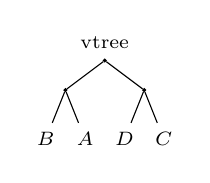
\begin{tikzpicture}[scale=0.5]
    \node[circle,draw=black,fill=black,inner sep=0,minimum width=0,label={above:\scriptsize vtree}] (root) at (0,0) {};
    \node[circle,draw=black,fill=black,inner sep=0,minimum width=0] (left) at (-1,-0.75) {};
    \node[circle,draw=black,fill=black,inner sep=0,minimum width=0] (right) at (1,-0.75) {};
    \draw (root) -- (left); \draw (root) -- (right);
    \node (B) at (-1.5,-2) {\scriptsize$B$};
    \draw (left) -- (B);
    \node (A) at (-0.5,-2) {\scriptsize$A$};
    \draw (left) -- (A);
    \node (D) at (0.5,-2) {\scriptsize$D$};
    \draw (right) -- (D);
    \node (C) at (1.5,-2) {\scriptsize$C$};
    \draw (right) -- (C);
  \end{tikzpicture}
  \hskip 0.25cm

  \vskip -2cm

  \only<4>{Partition...}
  \only<3>{Elements...}
  \only<2->{\vskip 0.5cm}

  \resizebox{0.9\textwidth}{!}{
  \begin{tikzpicture}[circuit logic US, every circuit symbol/.style={thick}]
    \begin{scope}[every node/.style={point up}]
      \newOrNode{r}{0,0}{}{inputs=nnn};
      \newAndNode{p1}{-1.5,-1.5}{}{inputs=nn};
      \newAndNode{p2}{0,-1.5}{}{inputs=nn};
      \newAndNode{p3}{2.0,-1.5}{}{inputs=nn};
      \newOrNode{s1}{-2.5,-3.0}{}{inputs=nn};
      \newOrNode{s2}{-0.25,-3.0}{}{inputs=nn};
      \newOrNode{s3}{3.0,-3.0}{}{inputs=nn};
      \newAndNode{q1}{-4.0,-4.5}{}{inputs=nn};
      \newAndNode{q2}{-1.875,-4.5}{}{inputs=nn};
      \newAndNode{q3}{0.25,-4.5}{}{inputs=nn};
      \newAndNode{q4}{2.375,-4.5}{}{inputs=nn};
      \newAndNode{q5}{4.5,-4.5}{}{inputs=nn};
    \end{scope}
    \begin{scope}[every node/.style={font=\Large}]
      \only<1,3->{
	\node (s1l1) at ($(p1.input 2) + (0,-1.0)$) {$D:\theta_D$};
	\node (s1l2) at ($(p2.input 2) + (0.75,-1.0)$) {$C$};
	\node (s1l3) at ($(p3.input 1) + (0,-1.0)$) {$\neg B$};
	\node (ql1) at ($(q1.input 1) + (-0.5,-1.0)$) {$B$};
	\node (ql2) at ($(q1.input 2) + (0.5, -1.0)$) {$A$};
	\node (ql3) at ($(q2.input 1) + (-0.5, -1.0)$) {$\neg B$};
	\node (ql5) at ($(q3.input 1) + (-0.5, -1.0)$) {$B$};
	\node (ql6) at ($(q3.input 2) + (0.5, -1.0)$) {$\neg A$};
	\node (ql7) at ($(q4.input 1) + (-0.5, -1.0)$) {$D$};
	\node (ql8) at ($(q4.input 2) + (0.5, -1.0)$) {$C$};
	\node (ql9) at ($(q5.input 1) + (-0.5, -1.0)$) {$\neg D$};
	\node (ql10) at ($(q5.input 2) + (0.5, -1.0)$) {$\bot$};
	\node (ql4) at ($(q2.input 2) + (0.5, -1.0)$) {$\bot$};
      }\only<2>{
	\node[palette1] (s1l1) at ($(p1.input 2) + (0,-1.0)$) {$D:\theta_D$};
	\node[palette2] (s1l2) at ($(p2.input 2) + (0.75,-1.0)$) {$C$};
	\node[palette2] (s1l3) at ($(p3.input 1) + (0,-1.0)$) {$\neg B$};
	\node[palette2] (ql1) at ($(q1.input 1) + (-0.5,-1.0)$) {$B$};
	\node[palette2] (ql2) at ($(q1.input 2) + (0.5, -1.0)$) {$A$};
	\node[palette2] (ql3) at ($(q2.input 1) + (-0.5, -1.0)$) {$\neg B$};
	\node[palette2] (ql5) at ($(q3.input 1) + (-0.5, -1.0)$) {$B$};
	\node[palette2] (ql6) at ($(q3.input 2) + (0.5, -1.0)$) {$\neg A$};
	\node[palette2] (ql7) at ($(q4.input 1) + (-0.5, -1.0)$) {$D$};
	\node[palette2] (ql8) at ($(q4.input 2) + (0.5, -1.0)$) {$C$};
	\node[palette2] (ql9) at ($(q5.input 1) + (-0.5, -1.0)$) {$\neg D$};
	\node[palette3] (ql10) at ($(q5.input 2) + (0.5, -1.0)$) {$\bot$};
	\node[palette3] (ql4) at ($(q2.input 2) + (0.5, -1.0)$) {$\bot$};
      }
    \end{scope}
    \only<2>{
      \node at ($(r)+(-2,0)$) {\large\color{blue!50!green!70}\textbf{OR gate}};
      \node at ($(p1)+(-2,0)$) {\large\color{blue!50!red!60}\textbf{AND gate}};
    }
    \draw (r.input 1) -- ++(0,-0.5) node[above left]{\footnotesize$0.35$} -| (p1);
    \draw (r.input 2) -- node[below right,xshift=.25cm,yshift=-.2cm]{\footnotesize$0.4$} (p2);
    \draw (r.input 3) -- ++(0,-0.5) node[above right]{\footnotesize$0.25$} -| (p3);
    \draw (s1.east) -- ++(0,0.25) -| (p1.input 1);
    \draw (s2.east) -- ++(0,0.25) -| (p2.input 1);
    \draw (s3.east) -- ++(0,0.25) -| (p3.input 2);
    \draw (s1l1) -- (p1.input 2);
    \draw (s1l2) -- ++(0,0.62) -| (p2.input 2);
    \draw (s1l3) -- (p3.input 1);
    \draw (q1.east) -- ++(0,0.25) -| node[above left]{\footnotesize$1.0$} (s1.input 1);
    \draw (q2.east) -- ++(0,0.25) -| node[above right]{\footnotesize$0.0$} (s1.input 2);
    \draw (q2.east) -- ++(0,0.25) -| node[above left]{\footnotesize$0.0$} (s2.input 1);
    \draw (q3.east) -- ++(0,0.25) -| node[above right]{\footnotesize$1.0$} (s2.input 2);
    \draw (q4.east) -- ++(0,0.25) -| node[above left]{\footnotesize$0.3$} (s3.input 1);
    \draw (q5.east) -- ++(0,0.25) -| node[above right]{\footnotesize$0.7$} (s3.input 2);
    \draw (q1.input 1) -- ++(0,-0.375) -| (ql1);
    \draw (q1.input 2) -- ++(0,-0.375) -| (ql2);
    \draw (q2.input 1) -- ++(0,-0.375) -| (ql3);
    \draw (q2.input 2) -- ++(0,-0.375) -| (ql4);
    \draw (q3.input 1) -- ++(0,-0.375) -| (ql5);
    \draw (q3.input 2) -- ++(0,-0.375) -| (ql6);
    \draw (q4.input 1) -- ++(0,-0.375) -| (ql7);
    \draw (q4.input 2) -- ++(0,-0.375) -| (ql8);
    \draw (q5.input 1) -- ++(0,-0.375) -| (ql9);
    \draw (q5.input 2) -- ++(0,-0.375) -| (ql10);
    \onslide<4>{
      \draw[draw=olive,thick] (-3.5,0.75) rectangle (3.60,-3.75);
    }
    \onslide<3>{
      \draw[draw=red,thick] (-3.0,-0.75) rectangle (-0.7,-3.75);
    }
  \end{tikzpicture}
  }
  \only<1>{
    \vskip 0.25cm
    \hfill\cite{kisa14}
  }
  \only<2>{
    \vskip 0.25cm
    \begin{center}
      Leaves are either \textcolor{palette2}{literals}, \textcolor{palette3}{constants} or
      \textcolor{palette1}{Bernoulli distributions}.
    \end{center}
  }
  \only<3-4>{
    \begin{equation*}
      \only<4>{\underbrace{(A\wedge B)}_{e_1}\vee\underbrace{((\neg A\wedge B)\wedge C)}_{e_2}\vee
      \underbrace{((C\wedge D)\wedge\neg B)}_{e_3}}
      \only<3>{\underbrace{(A\wedge B)}_\text{prime}\wedge\underbrace{(D\vee\neg D)}_\text{sub}}
    \end{equation*}
  }
\end{frame}

\iffull{
\begin{frame}
  \only<1>{Linear exact inference...}
  \vskip 0.5cm

  \resizebox{0.9\textwidth}{!}{
  \begin{tikzpicture}[circuit logic US, every circuit symbol/.style={thick}]
    \begin{scope}[every node/.style={point up}]
      \newOrNode{r}{0,0}{}{inputs=nnn};
      \newAndNode{p1}{-1.5,-1.5}{}{inputs=nn};
      \newAndNode{p2}{0,-1.5}{}{inputs=nn};
      \newAndNode{p3}{2.0,-1.5}{}{inputs=nn};
      \newOrNode{s1}{-2.5,-3.0}{}{inputs=nn};
      \newOrNode{s2}{-0.25,-3.0}{}{inputs=nn};
      \newOrNode{s3}{3.0,-3.0}{}{inputs=nn};
      \newAndNode{q1}{-4.0,-4.5}{}{inputs=nn};
      \newAndNode{q2}{-1.875,-4.5}{}{inputs=nn};
      \newAndNode{q3}{0.25,-4.5}{}{inputs=nn};
      \newAndNode{q4}{2.375,-4.5}{}{inputs=nn};
      \newAndNode{q5}{4.5,-4.5}{}{inputs=nn};
    \end{scope}
    \begin{scope}[every node/.style={font=\Large}]
      \node (s1l1) at ($(p1.input 2) + (0,-1.0)$) {$D:\theta_D$};
      \node (s1l2) at ($(p2.input 2) + (0.75,-1.0)$) {$C$};
      \node (s1l3) at ($(p3.input 1) + (0,-1.0)$) {$\neg B$};
      \node (ql1) at ($(q1.input 1) + (-0.5,-1.0)$) {$B$};
      \node (ql2) at ($(q1.input 2) + (0.5, -1.0)$) {$A$};
      \node (ql3) at ($(q2.input 1) + (-0.5, -1.0)$) {$\neg B$};
      \node (ql5) at ($(q3.input 1) + (-0.5, -1.0)$) {$B$};
      \node (ql6) at ($(q3.input 2) + (0.5, -1.0)$) {$\neg A$};
      \node (ql7) at ($(q4.input 1) + (-0.5, -1.0)$) {$D$};
      \node (ql8) at ($(q4.input 2) + (0.5, -1.0)$) {$C$};
      \node (ql9) at ($(q5.input 1) + (-0.5, -1.0)$) {$\neg D$};
      \node (ql10) at ($(q5.input 2) + (0.5, -1.0)$) {$\bot$};
      \node (ql4) at ($(q2.input 2) + (0.5, -1.0)$) {$\bot$};
    \end{scope}
    \only<1-5>{
      \draw (r.input 1) -- ++(0,-0.5) node[above left]{\footnotesize$0.35$} -| (p1);
      \draw (r.input 2) -- node[below right,xshift=.25cm,yshift=-.2cm]{\footnotesize$0.4$} (p2);
      \draw (r.input 3) -- ++(0,-0.5) node[above right]{\footnotesize$0.25$} -| (p3);
    }\only<1-4>{
      \draw (s1.east) -- ++(0,0.25) -| (p1.input 1);
      \draw (s2.east) -- ++(0,0.25) -| (p2.input 1);
      \draw (s3.east) -- ++(0,0.25) -| (p3.input 2);
      \draw (s1l1) -- (p1.input 2);
      \draw (s1l2) -- ++(0,0.62) -| (p2.input 2);
      \draw (s1l3) -- (p3.input 1);
    }\only<1-3>{
      \draw (q1.east) -- ++(0,0.25) -| node[above left]{\footnotesize$1.0$} (s1.input 1);
      \draw (q2.east) -- ++(0,0.25) -| node[above right]{\footnotesize$0.0$} (s1.input 2);
      \draw (q2.east) -- ++(0,0.25) -| node[above left]{\footnotesize$0.0$} (s2.input 1);
      \draw (q3.east) -- ++(0,0.25) -| node[above right]{\footnotesize$1.0$} (s2.input 2);
      \draw (q4.east) -- ++(0,0.25) -| node[above left]{\footnotesize$0.3$} (s3.input 1);
      \draw (q5.east) -- ++(0,0.25) -| node[above right]{\footnotesize$0.7$} (s3.input 2);
    }\only<1-2>{
      \draw (q1.input 1) -- ++(0,-0.375) -| (ql1);
      \draw (q1.input 2) -- ++(0,-0.375) -| (ql2);
      \draw (q2.input 1) -- ++(0,-0.375) -| (ql3);
      \draw (q2.input 2) -- ++(0,-0.375) -| (ql4);
      \draw (q3.input 1) -- ++(0,-0.375) -| (ql5);
      \draw (q3.input 2) -- ++(0,-0.375) -| (ql6);
      \draw (q4.input 1) -- ++(0,-0.375) -| (ql7);
      \draw (q4.input 2) -- ++(0,-0.375) -| (ql8);
      \draw (q5.input 1) -- ++(0,-0.375) -| (ql9);
      \draw (q5.input 2) -- ++(0,-0.375) -| (ql10);
    }\only<2->{
      \node[palette1] at ($(ql1) + (0,-0.5)$) {1};
      \node[palette1] at ($(ql2) + (0,-0.5)$) {0};
      \node[palette1] at ($(ql3) + (0,-0.5)$) {1};
      \node[palette1] at ($(ql4) + (0,-0.5)$) {0};
      \node[palette1] at ($(ql5) + (0,-0.5)$) {1};
      \node[palette1] at ($(ql6) + (0,-0.5)$) {1};
      \node[palette1] at ($(ql7) + (0,-0.5)$) {1};
      \node[palette1] at ($(ql8) + (0,-0.5)$) {1};
      \node[palette1] at ($(ql9) + (0,-0.5)$) {1};
      \node[palette1] at ($(ql10) + (0,-0.5)$) {0};
      \node[palette1] at ($(s1l1) + (0,-0.5)$) {1};
      \node[palette1] at ($(s1l2) + (0,-0.5)$) {1};
      \node[palette1] at ($(s1l3) + (0,-0.5)$) {1};
    }\only<3->{
      \draw[palette2] (q1.input 1) -- ++(0,-0.375) -| (ql1);
      \draw[palette2] (q1.input 2) -- ++(0,-0.375) -| (ql2);
      \draw[palette2] (q2.input 1) -- ++(0,-0.375) -| (ql3);
      \draw[palette2] (q2.input 2) -- ++(0,-0.375) -| (ql4);
      \draw[palette2] (q3.input 1) -- ++(0,-0.375) -| (ql5);
      \draw[palette2] (q3.input 2) -- ++(0,-0.375) -| (ql6);
      \draw[palette2] (q4.input 1) -- ++(0,-0.375) -| (ql7);
      \draw[palette2] (q4.input 2) -- ++(0,-0.375) -| (ql8);
      \draw[palette2] (q5.input 1) -- ++(0,-0.375) -| (ql9);
      \draw[palette2] (q5.input 2) -- ++(0,-0.375) -| (ql10);
      \node[black] at ($(q1.center)$) {0};
      \node[black] at ($(q2.center)$) {0};
      \node[black] at ($(q3.center)$) {1};
      \node[black] at ($(q4.center)$) {1};
      \node[black] at ($(q5.center)$) {0};
    }\only<4->{
      \draw[palette2] (q1.east) -- ++(0,0.25) -| node[above left]{\footnotesize$1.0$} (s1.input 1);
      \draw[palette2] (q2.east) -- ++(0,0.25) -| node[above right]{\footnotesize$0.0$} (s1.input 2);
      \draw[palette2] (q2.east) -- ++(0,0.25) -| node[above left]{\footnotesize$0.0$} (s2.input 1);
      \draw[palette2] (q3.east) -- ++(0,0.25) -| node[above right]{\footnotesize$1.0$} (s2.input 2);
      \draw[palette2] (q4.east) -- ++(0,0.25) -| node[above left]{\footnotesize$0.3$} (s3.input 1);
      \draw[palette2] (q5.east) -- ++(0,0.25) -| node[above right]{\footnotesize$0.7$} (s3.input 2);
      \node[black] at ($(s1.center)$) {0};
      \node[black] at ($(s2.center)$) {1};
      \node[black] at ($(s3.center)$) {\scriptsize 0.3};
    }\only<5->{
      \draw[palette2] (s1.east) -- ++(0,0.25) -| (p1.input 1);
      \draw[palette2] (s2.east) -- ++(0,0.25) -| (p2.input 1);
      \draw[palette2] (s3.east) -- ++(0,0.25) -| (p3.input 2);
      \draw[palette2] (s1l1) -- (p1.input 2);
      \draw[palette2] (s1l2) -- ++(0,0.62) -| (p2.input 2);
      \draw[palette2] (s1l3) -- (p3.input 1);
      \node[black] at ($(p1.center)$) {0};
      \node[black] at ($(p2.center)$) {1};
      \node[black] at ($(p3.center)$) {\scriptsize 0.3};
    }\only<6->{
      \draw[palette2] (r.input 1) -- ++(0,-0.5) node[above left]{\footnotesize$0.35$} -| (p1);
      \draw[palette2] (r.input 2) -- node[below right,xshift=.25cm,yshift=-.2cm]{\footnotesize$0.4$} (p2);
      \draw[palette2] (r.input 3) -- ++(0,-0.5) node[above right]{\footnotesize$0.25$} -| (p3);
      \node[black] at ($(r.center)$) {\scriptsize 0.475};
    }
  \end{tikzpicture}
  }
  \begin{equation*}
    \only<1-6>{P(A=0,C=1)=?}
    \only<7>{P(A=0,C=1)=0.475}
  \end{equation*}
\end{frame}
}

\section{Related Works}

\begin{frame}
  \frametitle{LearnPSDD}

  \textbf{Given.} A vtree and a circuit.
  \vskip 0.25cm

  \textbf{Idea.} Learn a PSDD as an expansion of initial circuit.
  \vskip 0.25cm

  \textbf{How?}
  \begin{enumerate}
    \item Recursively apply small changes;
    \item Evaluate score;
    \item Greedily accept changes.
  \end{enumerate}
  \vskip 0.5cm

  \begin{equation*}
    \text{Score}(\mathcal{S},\mathcal{S}'|D)=\frac{\log p(\mathcal{S}'|D) - \log
    p(\mathcal{S}|D)}{|\mathcal{S}'|-|\mathcal{S}|}
  \end{equation*}
  \vskip 0.5cm

  What are these ``small'' changes?
  \vskip 0.5cm

  \hfill\cite{liang17}
\end{frame}

\begin{frame}
  \only<1>{\textrm{\textsc{Split}} an element...}
  \only<2>{\textrm{\textsc{Clone}} a partition...}

  \only<1>{
    \begin{center}
      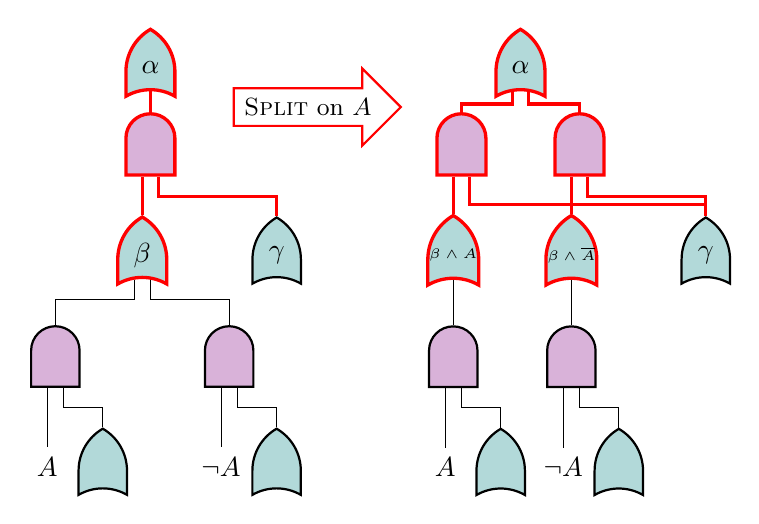
\begin{tikzpicture}[circuit logic US]
	\begin{scope}[every node/.style={point up}]
	  \begin{scope}[every circuit symbol/.style={draw=red,very thick}]
	    \newOrNode{r}{0,0}{$\alpha$}{inputs=nn};
	    \newAndNode{p1}{0,-1}{}{inputs=nn};
	    \newOrNode{s1}{$(p1.input 1) + (0,-1)$}{$\beta$}{inputs=nn};
	  \end{scope}
	  \begin{scope}[every circuit symbol/.style={thick}]
	    \newOrNode{s2}{$(p1.input 2) + (1.5,-1)$}{$\gamma$}{inputs=nn};
	    \newAndNode{p2}{$(s1.input 1) + (-1.0,-1)$}{}{inputs=nn};
	    \newAndNode{p3}{$(s1.input 2) + (1.0,-1)$}{}{inputs=nn};
	    \newOrNode{s3}{$(p2.input 2) + (0.5,-1)$}{}{inputs=nn};
	    \newOrNode{s4}{$(p3.input 2) + (0.5,-1)$}{}{inputs=nn};
	  \end{scope}
	\end{scope}
	\node (a) at ($(p2.input 1) + (0.0,-1)$) {$A$};
	\node (na) at ($(p3.input 1) + (0.0,-1)$) {$\neg A$};
	\draw[draw=red,very thick] (r.west) -- (p1.east);
	\draw[draw=red,very thick] (p1.input 1) -- (s1.east);
	\draw[draw=red,very thick] (p1.input 2) -- ++(0,-0.25) -| (s2.east);
	\draw (s1.input 1) -- ++(0,-0.25) -| (p2.east);
	\draw (s1.input 2) -- ++(0,-0.25) -| (p3.east);
	\draw (p2.input 1) -- (a);
	\draw (p2.input 2) -- ++(0,-0.25) -| (s3.east);
	\draw (p3.input 1) -- (na);
	\draw (p3.input 2) -- ++(0,-0.25) -| (s4.east);

	\node[style={single arrow,draw=red,thick}] (arrow) at (2,-0.5)
	  {\small\textrm{\textsc{Split}} on $A$};

	\begin{scope}[every node/.style={point up}]
	  \begin{scope}[every circuit symbol/.style={draw=red,very thick}]
	    \newOrNode{r}{$(arrow.east) + (1.5,0.5)$}{$\alpha$}{inputs=nn};
	    \newAndNode{p1}{$(r) + (0.75,-1)$}{}{inputs=nn};
	    \newAndNode{p12}{$(r) + (-0.75,-1)$}{}{inputs=nn};
	    \newOrNode{s1}{$(p1.input 1) + (0,-1)$}{\tiny$\beta\wedge\overline{A}$}{inputs=nn};
	    \newOrNode{s12}{$(p12.input 1) + (0,-1)$}{\tiny$\beta\wedge A$}{inputs=nn};
	  \end{scope}
	  \begin{scope}[every circuit symbol/.style={thick}]
	    \newOrNode{s2}{$(p1.input 2) + (1.5,-1)$}{$\gamma$}{inputs=nn};
	    \newAndNode{p2}{$(s12.west) + (0,-1)$}{}{inputs=nn};
	    \newAndNode{p3}{$(s1.west) + (0,-1)$}{}{inputs=nn};
	    \newOrNode{s3}{$(p2.input 2) + (0.5,-1)$}{}{inputs=nn};
	    \newOrNode{s4}{$(p3.input 2) + (0.5,-1)$}{}{inputs=nn};
	  \end{scope}
	\end{scope}
	\node (a) at ($(p2.input 1) + (0.0,-1)$) {$A$};
	\node (na) at ($(p3.input 1) + (0.0,-1)$) {$\neg A$};
	\draw[draw=red,very thick] (r.input 1) -- ++(0,-0.15) -| (p12.east);
	\draw[draw=red,very thick] (r.input 2) -- ++(0,-0.15) -| (p1.east);
	\draw[draw=red,very thick] (p1.input 1) -- (s1.east);
	\draw[draw=red,very thick] (p1.input 2) -- ++(0,-0.25) -| (s2.east);
	\draw[draw=red,very thick] (p12.input 2) -- ++(0,-0.35) -| (s2.east);
	\draw[draw=red,very thick] (p12.input 1) -- (s12.east);
	\draw (s12.west) -- ++(0,-0.25) -| (p2.east);
	\draw (s1.west) -- ++(0,-0.25) -| (p3.east);
	\draw (p2.input 1) -- (a);
	\draw (p2.input 2) -- ++(0,-0.25) -| (s3.east);
	\draw (p3.input 1) -- (na);
	\draw (p3.input 2) -- ++(0,-0.25) -| (s4.east);
      \end{tikzpicture}
    \end{center}
  }
  \only<2>{
    \begin{center}
      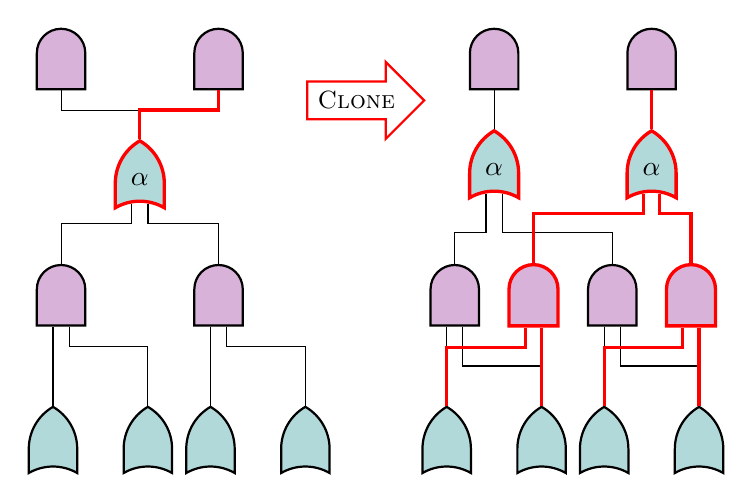
\begin{tikzpicture}[circuit logic US]
	\begin{scope}[every node/.style={point up}]
	  \begin{scope}[every circuit symbol/.style={draw=red,very thick}]
	    \newOrNode{s1}{0,-1.5}{$\alpha$}{inputs=nn};
	  \end{scope}
	  \begin{scope}[every circuit symbol/.style={thick}]
	    \newAndNode{r1}{-1,0}{}{inputs=nn};
	    \newAndNode{r2}{1,0}{}{inputs=nn};
	    \newAndNode{p1}{$(r1)+(0,-3)$}{}{inputs=nn};
	    \newAndNode{p2}{$(r2)+(0,-3)$}{}{inputs=nn};
	    \newOrNode{l11}{$(p1.input 1)+(0,-1.5)$}{}{inputs=nn};
	    \newOrNode{l12}{$(p1.input 2)+(1,-1.5)$}{}{inputs=nn};
	    \newOrNode{l21}{$(p2.input 1)+(0,-1.5)$}{}{inputs=nn};
	    \newOrNode{l22}{$(p2.input 2)+(1,-1.5)$}{}{inputs=nn};
	  \end{scope}
	\end{scope}
	\draw (r1.west) -- ++(0,-0.25) -| (s1.east);
	\draw[draw=red,very thick] (r2.west) -- ++(0,-0.25) -| (s1.east);
	\draw (s1.input 1) -- ++(0,-0.25) -| (p1.east);
	\draw (s1.input 2) -- ++(0,-0.25) -| (p2.east);
	\draw (p1.input 1) -- ++(0,-0.25) -| (l11.east);
	\draw (p1.input 2) -- ++(0,-0.25) -| (l12.east);
	\draw (p2.input 1) -- ++(0,-0.25) -| (l21.east);
	\draw (p2.input 2) -- ++(0,-0.25) -| (l22.east);

	\node[style={single arrow,draw=red,thick}] (arrow) at (2.75,-0.5)
	  {\small\textrm{\textsc{Clone}}};

	\begin{scope}[every node/.style={point up}]
	  \begin{scope}[every circuit symbol/.style={thick}]
	    \newAndNode{r1}{4.5,0}{}{inputs=nn};
	    \newAndNode{r2}{6.5,0}{}{inputs=nn};
	    \newAndNode{p1}{$(r1)+(-0.5,-3)$}{}{inputs=nn};
	    \newAndNode{p2}{$(r2)+(-0.5,-3)$}{}{inputs=nn};
	    \newOrNode{l11}{$(p1.input 1)+(0,-1.5)$}{}{inputs=nn};
	    \newOrNode{l12}{$(p1.input 2)+(1,-1.5)$}{}{inputs=nn};
	    \newOrNode{l21}{$(p2.input 1)+(0,-1.5)$}{}{inputs=nn};
	    \newOrNode{l22}{$(p2.input 2)+(1,-1.5)$}{}{inputs=nn};
	  \end{scope}
	  \begin{scope}[every circuit symbol/.style={draw=red,very thick}]
	    \newOrNode{s1}{$(r1.west) + (0,-1)$}{$\alpha$}{inputs=nn};
	    \newOrNode{s2}{$(r2.west) + (0,-1)$}{$\alpha$}{inputs=nn};
	    \newAndNode{p3}{$(p1)+(1,0)$}{}{inputs=nn};
	    \newAndNode{p4}{$(p2)+(1,0)$}{}{inputs=nn};
	  \end{scope}
	\end{scope}
	\draw (r1.west) -- ++(0,-0.25) -| (s1.east);
	\draw[draw=red,very thick] (r2.west) -- ++(0,-0.25) -| (s2.east);
	\draw (s1.input 1) -- ++(0,-0.5) -| (p1.east);
	\draw (s1.input 2) -- ++(0,-0.5) -| (p2.east);
	\draw[draw=red,very thick] (s2.input 1) -- ++(0,-0.25) -| (p3.east);
	\draw[draw=red,very thick] (s2.input 2) -- ++(0,-0.25) -| (p4.east);
	\draw (p1.input 1) -- ++(0,-0.25) -| (l11.east);
	\draw (p1.input 2) -- ++(0,-0.5) -| (l12.east);
	\draw (p2.input 1) -- ++(0,-0.25) -| (l21.east);
	\draw (p2.input 2) -- ++(0,-0.5) -| (l22.east);
	\draw[draw=red,very thick] (p3.input 1) -- ++(0,-0.25) -| (l11.east);
	\draw[draw=red,very thick] (p3.input 2) -- ++(0,-0.5) -| (l12.east);
	\draw[draw=red,very thick] (p4.input 1) -- ++(0,-0.25) -| (l21.east);
	\draw[draw=red,very thick] (p4.input 2) -- ++(0,-0.5) -| (l22.east);
      \end{tikzpicture}
    \end{center}
  }
\end{frame}

\begin{frame}
  \frametitle{Strudel}

  \textbf{Given.} A Chow-Liu Tree (CLT).
  \vskip 0.5cm

  \textbf{Idea.} Learn a PSDD and its vtree.
  \vskip 0.5cm

  \textbf{How?}
  \begin{enumerate}
    \item Learn a CLT.
    \item Extract a vtree from CLT.
    \item Compile CLT into circuit.
    \item ``Grow'' circuit with \textrm{\textsc{Split}}.
  \end{enumerate}
  \vskip 0.5cm

  \hfill\cite{dang20}
\end{frame}

\begin{frame}
  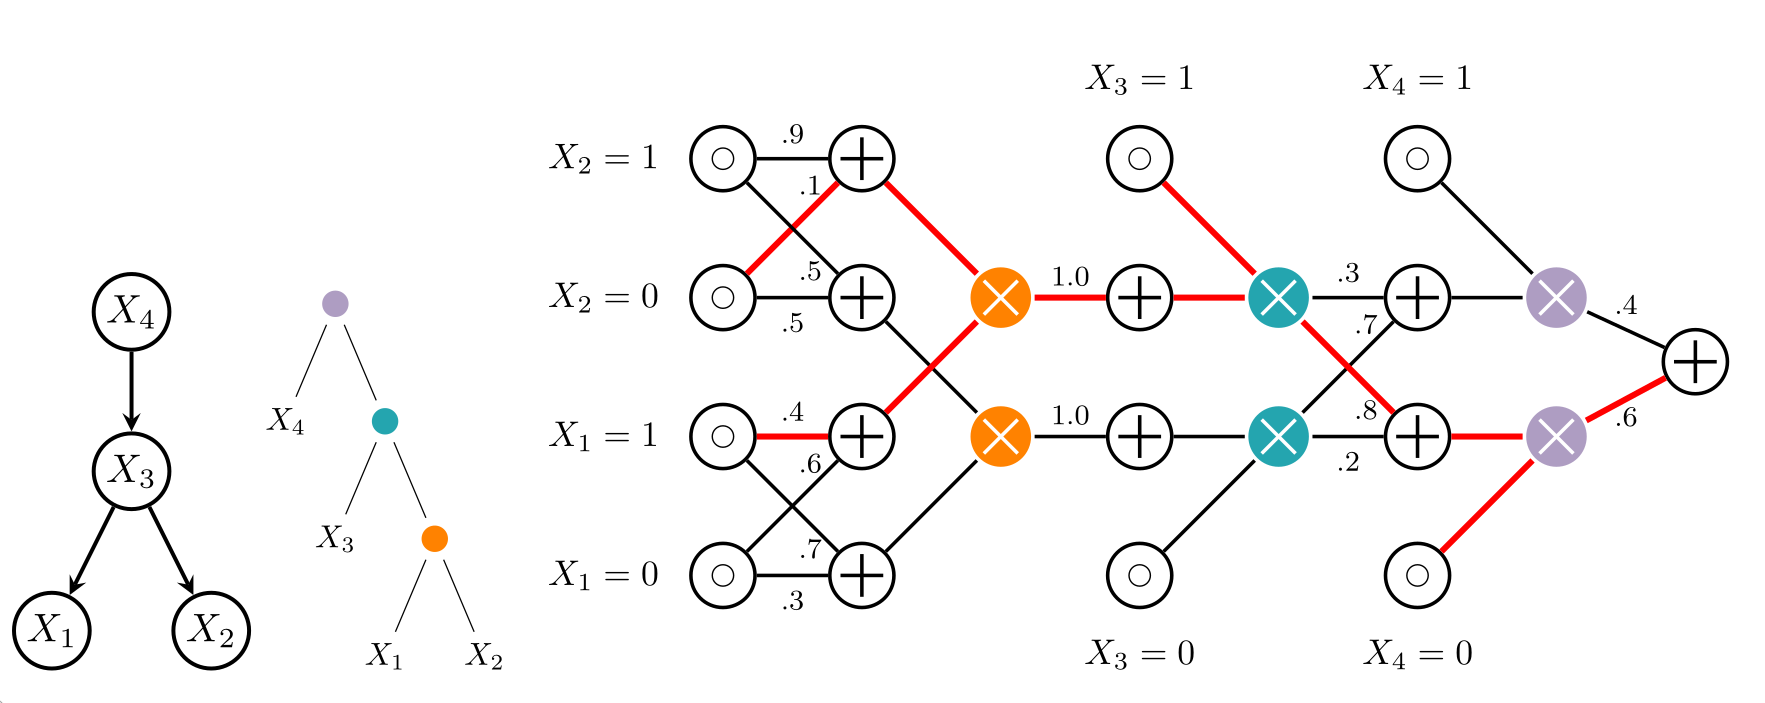
\includegraphics[width=\textwidth]{imgs/strudel.png}
  \vskip 1.0cm
  \hfill\cite{dang20}
\end{frame}

\section{Learning by Sampling}

\begin{frame}
  \frametitle{Monte-Carlo Structure Learning}

  Previous attempts \emph{grew} or \emph{compiled} existing models.
  \vskip 0.5cm
  Instead, we want to \emph{build} a circuit solely from knowledge.
  \vskip 0.5cm

  \textbf{Our approach.} Start off with a logic formula:

  \begin{equation*}
    \scriptstyle
    \phi(A,B,C,D,E)=(B\wedge C\wedge((A\wedge D\wedge\neg E)\vee(\neg A\wedge E)))\vee(\neg A\wedge
    ((\neg C\wedge D\wedge\neg E)\vee\neg B))
  \end{equation*}
  \vskip 0.5cm

  Recursively decompose $\phi$ top-down through subsequent partitions.
\end{frame}

\begin{frame}
  \hfill\begin{tikzpicture}[scale=0.5,yshift=-3cm]
    \node[circle,draw=black,fill=black,inner sep=0,minimum width=0,label={above:\scriptsize vtree}] (root) at (0,0) {};
    \node[circle,draw=black,fill=black,inner sep=0,minimum width=0] (left) at (-1,-0.75) {};
    \node[circle,draw=black,fill=black,inner sep=0,minimum width=0] (right) at (1,-0.75) {};
    \node[circle,draw=black,fill=black,inner sep=0,minimum width=0] (left2) at (-0.5,-2) {};
    \draw (root) -- (left); \draw (root) -- (right);
    \draw (left) -- (left2);
    \node (A) at (-1.0,-3.25) {\scriptsize$A$};
    \node (B) at (-0.0,-3.25) {\scriptsize$B$};
    \draw (left2) -- (B); \draw (left2) -- (A);
    \node (C) at (-1.5,-2) {\scriptsize$C$};
    \draw (left) -- (C);
    \node (D) at (0.5,-2) {\scriptsize$D$};
    \node (E) at (1.5,-2) {\scriptsize$E$};
    \draw (right) -- (E); \draw (right) -- (D);
    \node (tmp) at (-10,0) {};
  \end{tikzpicture}

  \vskip -1.0cm
  How to decompose formula into elements...

  \begin{equation*}
    (B\wedge C\wedge((A\wedge D\wedge\neg E)\vee(\neg A\wedge E)))\vee(\neg A\wedge ((\neg C\wedge
    D\wedge\neg E)\vee\neg B))
  \end{equation*}
  \resizebox{\textwidth}{!}{
  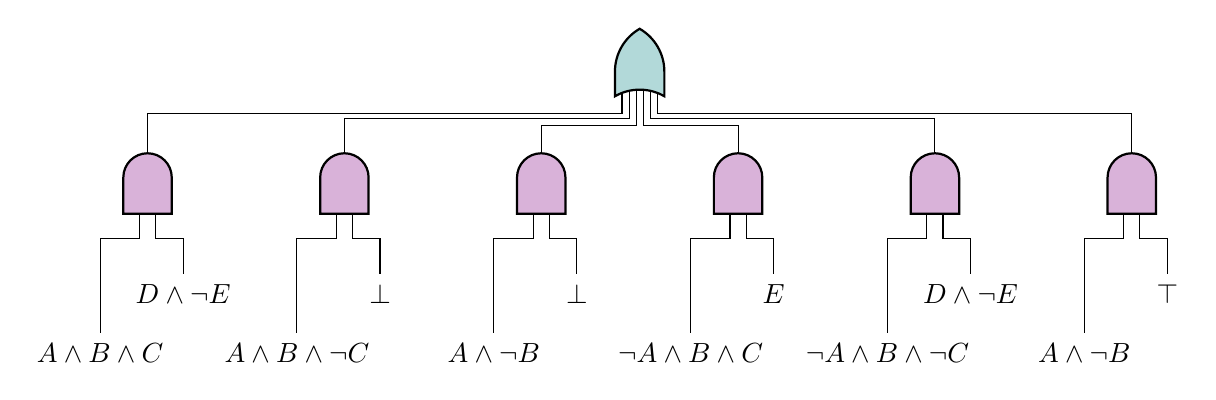
\begin{tikzpicture}[circuit logic US,every circuit symbol/.style={thick,point up}]
    \newOrNode{r}{0,0}{}{scale=0.5,inputs=nnnnnn};
    \newAndNode{e1}{$(r)+(-6.25,-1.5)$}{}{inputs=nn};
    \newAndNode{e2}{$(r)+(-3.75,-1.5)$}{}{inputs=nn};
    \newAndNode{e3}{$(r)+(-1.25,-1.5)$}{}{inputs=nn};
    \newAndNode{e4}{$(r)+(1.25,-1.5)$}{}{inputs=nn};
    \newAndNode{e5}{$(r)+(3.75,-1.5)$}{}{inputs=nn};
    \newAndNode{e6}{$(r)+(6.25,-1.5)$}{}{inputs=nn};
    \draw (r.input 1) -- ++(0,-0.25) -| (e1.east);
    \draw (r.input 2) -- ++(0,-0.35) -| (e2.east);
    \draw (r.input 3) -- ++(0,-0.45) -| (e3.east);
    \draw (r.input 4) -- ++(0,-0.45) -| (e4.east);
    \draw (r.input 5) -- ++(0,-0.35) -| (e5.east);
    \draw (r.input 6) -- ++(0,-0.25) -| (e6.east);
    \node (p1) at ($(e1.input 1) + (-0.5,-1.75)$) {$A\wedge B\wedge C$};
    \node (s1) at ($(e1.input 2) + (0.35,-1.0)$) {$D\wedge\neg E$};
    \draw (e1.input 1) -- ++(0,-0.3) -| (p1);
    \draw (e1.input 2) -- ++(0,-0.3) -| (s1);
    \node (p2) at ($(e2.input 1) + (-0.5,-1.75)$) {$A\wedge B\wedge\neg C$};
    \node (s2) at ($(e2.input 2) + (0.35,-1.0)$) {$\bot$};
    \draw (e2.input 1) -- ++(0,-0.3) -| (p2);
    \draw (e2.input 2) -- ++(0,-0.3) -| (s2);
    \node (p3) at ($(e3.input 1) + (-0.5,-1.75)$) {$A\wedge\neg B$};
    \node (s3) at ($(e3.input 2) + (0.35,-1.0)$) {$\bot$};
    \draw (e3.input 1) -- ++(0,-0.3) -| (p3);
    \draw (e3.input 2) -- ++(0,-0.3) -| (s3);
    \node (p4) at ($(e4.input 1) + (-0.5,-1.75)$) {$\neg A\wedge B\wedge C$};
    \node (s4) at ($(e4.input 2) + (0.35,-1.0)$) {$E$};
    \draw (e4.input 1) -- ++(0,-0.3) -| (p4);
    \draw (e4.input 2) -- ++(0,-0.3) -| (s4);
    \node (p5) at ($(e5.input 1) + (-0.5,-1.75)$) {$\neg A\wedge B\wedge\neg C$};
    \node (s5) at ($(e5.input 2) + (0.35,-1.0)$) {$D\wedge\neg E$};
    \draw (e5.input 1) -- ++(0,-0.3) -| (p5);
    \draw (e5.input 2) -- ++(0,-0.3) -| (s5);
    \node (p6) at ($(e6.input 1) + (-0.5,-1.75)$) {$A\wedge\neg B$};
    \node (s6) at ($(e6.input 2) + (0.35,-1.0)$) {$\top$};
    \draw (e6.input 1) -- ++(0,-0.3) -| (p6);
    \draw (e6.input 2) -- ++(0,-0.3) -| (s6);
  \end{tikzpicture}
  }
  \vskip 0.75cm
  \hfill ...while ensuring primes are exhaustive and mutually exclusive?
\end{frame}

\begin{frame}
  Given a prime ordering, such as $\set{O}=(B,C,A)$, return a set of primes.
  \vskip 0.5cm

  \onslide<2->{
  \centering
  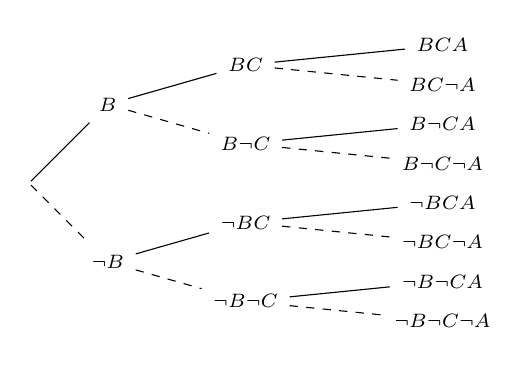
\begin{tikzpicture}
    \begin{scope}[every node/.style={inner sep=4pt,font=\scriptsize}]
      \node[inner sep=0pt] (e) at (0, 0) {};
      \node (b) at (1.0, 1.0) {$B$};
      \node (nb) at (1.0, -1.0) {$\neg B$};
      \onslide<3->{
      \node (bc) at (2.75, 1.5) {$BC$};
      \node (bnc) at (2.75, 0.5) {$B\neg C$};
      \node (nbc) at (2.75, -0.5) {$\neg BC$};
      \node (nbnc) at (2.75, -1.5) {$\neg B\neg C$};
      \onslide<4->{
      \node (bca) at (5.25, 1.75) {$BCA$};
      \node (bcna) at (5.25, 1.25) {$BC\neg A$};
      \node (nbca) at (5.25, -0.25) {$\neg BCA$};
      \node (nbcna) at (5.25, -0.75) {$\neg BC\neg A$};
      \node (bnca) at (5.25, 0.75) {$B\neg CA$};
      \node (bncna) at (5.25, 0.25) {$B\neg C\neg A$};
      \node (nbnca) at (5.25, -1.25) {$\neg B\neg CA$};
      \node (nbncna) at (5.25, -1.75) {$\neg B\neg C\neg A$};
      }}
    \end{scope}
    \draw (e) -- (b);
    \draw[dashed] (e) -- (nb);
    \onslide<3->{
    \draw[dashed] (b) -- (bnc);
    \draw (b) -- (bc);
    \draw (nb) -- (nbc);
    \draw[dashed] (nb) -- (nbnc);
    \onslide<4->{
    \draw (bc) -- (bca);
    \draw[dashed] (bc) -- (bcna);
    \draw (nbc) -- (nbca);
    \draw[dashed] (nbc) -- (nbcna);
    \draw (bnc) -- (bnca);
    \draw[dashed] (bnc) -- (bncna);
    \draw (nbnc) -- (nbnca);
    \draw[dashed] (nbnc) -- (nbncna);
    }}
  \end{tikzpicture}
  }
  \vskip 0.5cm
  \only<5>{This gives an exponential number of elements!}
\end{frame}

\begin{frame}
  Instead, let's ``forget'' a variable when it does not ``matter'', i.e. when
  \begin{equation*}
    \phi|_x=\phi|_{\neg x}.
  \end{equation*}
  \vskip 0.5cm
  \onslide<2->{
  \centering
  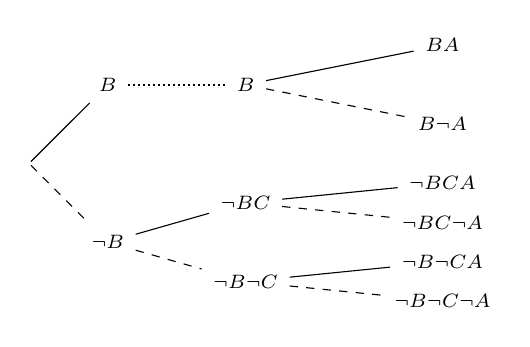
\begin{tikzpicture}
    \begin{scope}[every node/.style={inner sep=4pt,font=\scriptsize}]
      \node[inner sep=0pt] (e) at (0, 0) {};
      \node (b) at (1.0, 1.0) {$B$};
      \node (nb) at (1.0, -1.0) {$\neg B$};
      \onslide<3->{
      \node (bmc) at (2.75, 1.0) {$B$};
      \node (nbc) at (2.75, -0.5) {$\neg BC$};
      \node (nbnc) at (2.75, -1.5) {$\neg B\neg C$};
      \onslide<4->{
      \node (ba) at (5.25, 1.5) {$BA$};
      \node (bna) at (5.25, 0.5) {$B\neg A$};
      \node (nbca) at (5.25, -0.25) {$\neg BCA$};
      \node (nbcna) at (5.25, -0.75) {$\neg BC\neg A$};
      \node (nbnca) at (5.25, -1.25) {$\neg B\neg CA$};
      \node (nbncna) at (5.25, -1.75) {$\neg B\neg C\neg A$};
      }}
    \end{scope}
    \draw (e) -- (b);
    \draw[dashed] (e) -- (nb);
    \onslide<3->{
    \draw[thick,densely dotted] (b) -- (bmc);
    \draw (nb) -- (nbc);
    \draw[dashed] (nb) -- (nbnc);
    \onslide<4->{
    \draw (bmc) -- (ba);
    \draw[dashed] (bmc) -- (bna);
    \draw (nbc) -- (nbca);
    \draw[dashed] (nbc) -- (nbcna);
    \draw (nbnc) -- (nbnca);
    \draw[dashed] (nbnc) -- (nbncna);
    }}
  \end{tikzpicture}
  }
  \vskip 0.5cm
  \only<5>{We avoid computing an exponential number of primes!}
\end{frame}

\begin{frame}
  In other words...
  \vskip 0.5cm

  \textbf{Given.}
  \begin{itemize}
    \item A random prime ordering $\set{O}=\{X_1,\ldots,X_n\}$;
    \item A formula $\phi$.
  \end{itemize}
  \vskip 0.5cm

  Generate a set of primes $\{p_i\}_{i=1}^n$, and then subs $s_i=\phi|_{p_i}$.
  \vskip 0.5cm

  But what if $\phi\equiv\top$ or $\forall X_i\in\set{O}$, $X_i\not\in\phi$?
\end{frame}

\begin{frame}
  Then we have even more freedom! Stochastically marginalize with some probability $p$.
  \vskip 0.5cm

  \begin{center}
    \begin{tikzpicture}
      \only<1>{
      \begin{scope}[every node/.style={inner sep=4pt,font=\scriptsize}]
	\node[inner sep=0pt] (e) at (0, 0) {};
	\node (b) at (1.0, 1.0) {$B$};
	\node (nb) at (1.0, -1.0) {$\neg B$};
	\node (bmc) at (2.75, 1.0) {$B$};
	\node (nbc) at (2.75, -0.5) {$\neg BC$};
	\node (nbnc) at (2.75, -1.5) {$\neg B\neg C$};
	\node (ba) at (5.25, 1.5) {$BA$};
	\node (bna) at (5.25, 0.5) {$B\neg A$};
	\node (nbca) at (5.25, -0.25) {$\neg BCA$};
	\node (nbcna) at (5.25, -0.75) {$\neg BC\neg A$};
	\node (nbnca) at (5.25, -1.25) {$\neg B\neg CA$};
	\node (nbncna) at (5.25, -1.75) {$\neg B\neg C\neg A$};
      \end{scope}
      \draw (e) -- (b);
      \draw[dashed] (e) -- (nb);
      \draw[thick,densely dotted] (b) -- (bmc);
      \draw (nb) -- (nbc);
      \draw[dashed] (nb) -- (nbnc);
      \draw (bmc) -- (ba);
      \draw[dashed] (bmc) -- (bna);
      \draw (nbc) -- (nbca);
      \draw[dashed] (nbc) -- (nbcna);
      \draw (nbnc) -- (nbnca);
      \draw[dashed] (nbnc) -- (nbncna);
      }\only<2>{
      \begin{scope}[every node/.style={inner sep=4pt,font=\scriptsize}]
	\node[inner sep=0pt] (e) at (0, 0) {};
	\node (b) at (1.0, 1.0) {$C$};
	\node (nb) at (1.0, -1.0) {$\neg C$};
	\node (bc) at (2.75, 1.5) {$CA$};
	\node (bnc) at (2.75, 0.5) {$C\neg A$};
	\node (nbc) at (2.75, -0.5) {$\neg CA$};
	\node (nbnc) at (2.75, -1.5) {$\neg C\neg A$};
      \end{scope}
      \draw (e) -- (b);
      \draw[dashed] (e) -- (nb);
      \draw[dashed] (b) -- (bnc);
      \draw (b) -- (bc);
      \draw (nb) -- (nbc);
      \draw[dashed] (nb) -- (nbnc);
      }
    \end{tikzpicture}
  \end{center}
  \vskip 0.5cm

  We can marginalize any variable we want, since any operation on $\phi$ with $X_i$ is idempotent.
\end{frame}

\begin{frame}
  \only<1,2,4,5>{
    \begin{equation*}
      (B\wedge C\wedge((A\wedge D\wedge\neg E)\vee(\neg A\wedge E)))\vee(\neg A\wedge ((\neg C\wedge
      D\wedge\neg E)\vee\neg B))
    \end{equation*}
    \resizebox{\textwidth}{!}{
    \begin{tikzpicture}[circuit logic US,every circuit symbol/.style={thick,point up}]
      \only<1>{
      \newOrNode{r}{0,0}{}{scale=0.5,inputs=nnnnnn};
      \newAndNode{e1}{$(r)+(-6.25,-1.5)$}{}{inputs=nn};
      \newAndNode{e2}{$(r)+(-3.75,-1.5)$}{}{inputs=nn};
      \newAndNode{e3}{$(r)+(-1.25,-1.5)$}{}{inputs=nn};
      \newAndNode{e4}{$(r)+(1.25,-1.5)$}{}{inputs=nn};
      \newAndNode{e5}{$(r)+(3.75,-1.5)$}{}{inputs=nn};
      \newAndNode{e6}{$(r)+(6.25,-1.5)$}{}{inputs=nn};
      \draw (r.input 1) -- ++(0,-0.25) -| (e1.east);
      \draw (r.input 2) -- ++(0,-0.35) -| (e2.east);
      \draw (r.input 3) -- ++(0,-0.45) -| (e3.east);
      \draw (r.input 4) -- ++(0,-0.45) -| (e4.east);
      \draw (r.input 5) -- ++(0,-0.35) -| (e5.east);
      \draw (r.input 6) -- ++(0,-0.25) -| (e6.east);
      \node (p1) at ($(e1.input 1) + (-0.5,-1.75)$) {$A\wedge B\wedge C$};
      \node (s1) at ($(e1.input 2) + (0.35,-1.0)$) {$D\wedge\neg E$};
      \draw (e1.input 1) -- ++(0,-0.3) -| (p1);
      \draw (e1.input 2) -- ++(0,-0.3) -| (s1);
      \node (p2) at ($(e2.input 1) + (-0.5,-1.75)$) {$A\wedge B\wedge\neg C$};
      \node (s2) at ($(e2.input 2) + (0.35,-1.0)$) {$\bot$};
      \draw (e2.input 1) -- ++(0,-0.3) -| (p2);
      \draw (e2.input 2) -- ++(0,-0.3) -| (s2);
      \node (p3) at ($(e3.input 1) + (-0.5,-1.75)$) {$A\wedge\neg B$};
      \node (s3) at ($(e3.input 2) + (0.35,-1.0)$) {$\bot$};
      \draw (e3.input 1) -- ++(0,-0.3) -| (p3);
      \draw (e3.input 2) -- ++(0,-0.3) -| (s3);
      \node (p4) at ($(e4.input 1) + (-0.5,-1.75)$) {$\neg A\wedge B\wedge C$};
      \node (s4) at ($(e4.input 2) + (0.35,-1.0)$) {$E$};
      \draw (e4.input 1) -- ++(0,-0.3) -| (p4);
      \draw (e4.input 2) -- ++(0,-0.3) -| (s4);
      \node (p5) at ($(e5.input 1) + (-0.5,-1.75)$) {$\neg A\wedge B\wedge\neg C$};
      \node (s5) at ($(e5.input 2) + (0.35,-1.0)$) {$D\wedge\neg E$};
      \draw (e5.input 1) -- ++(0,-0.3) -| (p5);
      \draw (e5.input 2) -- ++(0,-0.3) -| (s5);
      \node (p6) at ($(e6.input 1) + (-0.5,-1.75)$) {$A\wedge\neg B$};
      \node (s6) at ($(e6.input 2) + (0.35,-1.0)$) {$\top$};
      \draw (e6.input 1) -- ++(0,-0.3) -| (p6);
      \draw (e6.input 2) -- ++(0,-0.3) -| (s6);
      }\only<2>{
      \newOrNode{r}{0,0}{}{inputs=nnnn};
      \newAndNode{e1}{$(r)+(-5,-1.5)$}{}{inputs=nn};
      \newAndNode{e4}{$(r)+(-1.67,-1.5)$}{}{inputs=nn};
      \newAndNode{e5}{$(r)+(1.67,-1.5)$}{}{inputs=nn};
      \newAndNode{e6}{$(r)+(5,-1.5)$}{}{inputs=nn};
      \draw (r.input 1) -- ++(0,-0.25) -| (e1.east);
      \draw (r.input 2) -- ++(0,-0.5) -| (e4.east);
      \draw (r.input 3) -- ++(0,-0.5) -| (e5.east);
      \draw (r.input 4) -- ++(0,-0.25) -| (e6.east);
      \node (p1) at ($(e1.input 1) + (-0.5,-1.75)$) {$A\wedge B\wedge C$};
      \node (s1) at ($(e1.input 2) + (0.35,-1.0)$) {$D\wedge\neg E$};
      \draw (e1.input 1) -- ++(0,-0.3) -| (p1);
      \draw (e1.input 2) -- ++(0,-0.3) -| (s1);
      \node (p4) at ($(e4.input 1) + (-0.5,-1.75)$) {$\neg A\wedge B\wedge C$};
      \node (s4) at ($(e4.input 2) + (0.35,-1.0)$) {$E$};
      \draw (e4.input 1) -- ++(0,-0.3) -| (p4);
      \draw (e4.input 2) -- ++(0,-0.3) -| (s4);
      \node (p5) at ($(e5.input 1) + (-0.5,-1.75)$) {$\neg A\wedge B\wedge\neg C$};
      \node (s5) at ($(e5.input 2) + (0.35,-1.0)$) {$D\wedge\neg E$};
      \draw (e5.input 1) -- ++(0,-0.3) -| (p5);
      \draw (e5.input 2) -- ++(0,-0.3) -| (s5);
      \node (p6) at ($(e6.input 1) + (-0.5,-1.75)$) {$A\wedge\neg B$};
      \node (s6) at ($(e6.input 2) + (0.35,-1.0)$) {$\top$};
      \draw (e6.input 1) -- ++(0,-0.3) -| (p6);
      \draw (e6.input 2) -- ++(0,-0.3) -| (s6);
      }\only<4>{
      \newOrNode{r}{0,0}{}{inputs=nnnn};
      \newAndNode{e1}{$(r)+(-5,-1.5)$}{}{inputs=nn};
      \newAndNode{e4}{$(r)+(-1.67,-1.5)$}{}{inputs=nn};
      \newAndNode{e5}{$(r)+(1.67,-1.5)$}{}{inputs=nn};
      \newAndNode{e6}{$(r)+(5,-1.5)$}{}{inputs=nn};
      \draw (r.input 1) -- ++(0,-0.25) -| (e1.east);
      \draw (r.input 2) -- ++(0,-0.5) -| (e4.east);
      \draw (r.input 3) -- ++(0,-0.5) -| (e5.east);
      \draw (r.input 4) -- ++(0,-0.25) -| (e6.east);
      \node (p1) at ($(e1.input 1) + (-0.5,-1.75)$) {$A\wedge B\wedge C$};
      \node (s1) at ($(e1.input 2) + (0.35,-1.0)$) {$D\wedge\neg E$};
      \draw (e1.input 1) -- ++(0,-0.3) -| (p1);
      \draw (e1.input 2) -- ++(0,-0.3) -| (s1);
      \node (p4) at ($(e4.input 1) + (-0.5,-1.75)$) {$\neg A\wedge B\wedge\neg C$};
      \node (s4) at ($(e4.input 2) + (0.35,-1.0)$) {$D\wedge\neg E$};
      \draw (e4.input 1) -- ++(0,-0.3) -| (p4);
      \draw (e4.input 2) -- ++(0,-0.3) -| (s4);
      \node (p5) at ($(e5.input 1) + (-0.5,-1.75)$) {$\neg A\wedge B\wedge C$};
      \node (s5) at ($(e5.input 2) + (0.35,-1.0)$) {$E$};
      \draw (e5.input 1) -- ++(0,-0.3) -| (p5);
      \draw (e5.input 2) -- ++(0,-0.3) -| (s5);
      \node (p6) at ($(e6.input 1) + (-0.5,-1.75)$) {$A\wedge\neg B$};
      \node (s6) at ($(e6.input 2) + (0.35,-1.0)$) {$\top$};
      \draw (e6.input 1) -- ++(0,-0.3) -| (p6);
      \draw (e6.input 2) -- ++(0,-0.3) -| (s6);
      }\only<5>{
      \newOrNode{r}{0,0}{}{inputs=nnn};
      \newAndNode{e4}{$(r)+(-3.35,-1.5)$}{}{inputs=nn};
      \newAndNode{e5}{$(r)+(1.67,-1.5)$}{}{inputs=nn};
      \newAndNode{e6}{$(r)+(5,-1.5)$}{}{inputs=nn};
      \draw (r.input 1) -- ++(0,-0.25) -| (e4.east);
      \draw (r.input 2) -- ++(0,-0.5) -| (e5.east);
      \draw (r.input 3) -- ++(0,-0.25) -| (e6.east);
      \node (p4) at ($(e4.input 1) + (-1.0,-1.75)$) {$(\neg A\wedge B\wedge\neg C)\vee(\neg A\wedge B
	\wedge\neg C)$};
      \node (s4) at ($(e4.input 2) + (0.35,-1.0)$) {$D\wedge\neg E$};
      \draw (e4.input 1) -- ++(0,-0.3) -| (p4);
      \draw (e4.input 2) -- ++(0,-0.3) -| (s4);
      \node (p5) at ($(e5.input 1) + (-0.5,-1.75)$) {$\neg A\wedge B\wedge C$};
      \node (s5) at ($(e5.input 2) + (0.35,-1.0)$) {$E$};
      \draw (e5.input 1) -- ++(0,-0.3) -| (p5);
      \draw (e5.input 2) -- ++(0,-0.3) -| (s5);
      \node (p6) at ($(e6.input 1) + (-0.5,-1.75)$) {$A\wedge\neg B$};
      \node (s6) at ($(e6.input 2) + (0.35,-1.0)$) {$\top$};
      \draw (e6.input 1) -- ++(0,-0.3) -| (p6);
      \draw (e6.input 2) -- ++(0,-0.3) -| (s6);
      }
    \end{tikzpicture}
    }
  }\only<3>{
    \frametitle{Compression}

    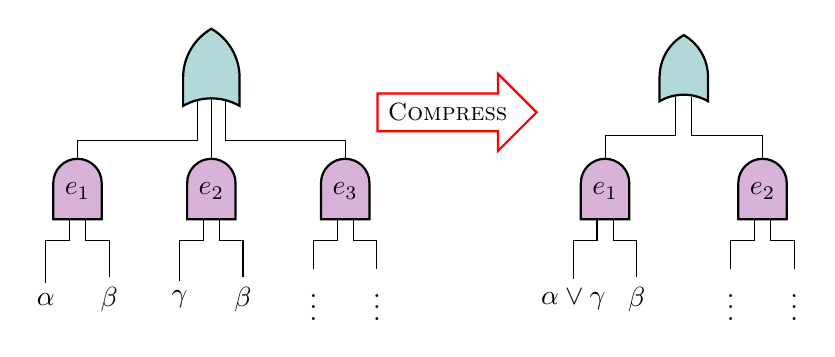
\begin{tikzpicture}[circuit logic US, every circuit symbol/.style={thick}]
      \begin{scope}[every node/.style={point up}]
	\newOrNode{r}{0,0}{}{inputs=nnn};
	\newAndNode{q1}{$(r)+(-1.7,-1.5)$}{$e_1$}{inputs=nn};
	\newAndNode{q2}{$(r)+(0.0,-1.5)$}{$e_2$}{inputs=nn};
	\newAndNode{q3}{$(r)+(1.7,-1.5)$}{$e_3$}{inputs=nn};
      \end{scope}
      \node (p1) at ($(q1.input 1) + (-0.3,-1.0)$) {$\alpha$};
      \node (s1) at ($(q1.input 2) + (0.3,-1.0)$) {$\beta$};
      \node (p2) at ($(q2.input 1) + (-0.3,-1.0)$) {$\gamma$};
      \node (s2) at ($(q2.input 2) + (0.3,-1.0)$) {$\beta$};
      \node (p3) at ($(q3.input 1) + (-0.3,-1.0)$) {$\vdots$};
      \node (s3) at ($(q3.input 2) + (0.3,-1.0)$) {$\vdots$};
      \draw (r.input 1) -- ++(0,-0.5) -| (q1.east);
      \draw (r.input 2) -- ++(0,-0.5) -| (q2.east);
      \draw (r.input 3) -- ++(0,-0.5) -| (q3.east);
      \draw (q1.input 1) -- ++(0,-0.25) -| (p1);
      \draw (q1.input 2) -- ++(0,-0.25) -| (s1);
      \draw (q2.input 1) -- ++(0,-0.25) -| (p2);
      \draw (q2.input 2) -- ++(0,-0.25) -| (s2);
      \draw (q3.input 1) -- ++(0,-0.25) -| (p3);
      \draw (q3.input 2) -- ++(0,-0.25) -| (s3);

      \node[style={single arrow,draw=red,thick}] (arrow) at (3,-0.5)
	{\small\textrm{\textsc{Compress}}};

      \begin{scope}[every node/.style={point up}]
	\newOrNode{r}{6,0}{}{inputs=nn};
	\newAndNode{q1}{$(r)+(-1.0,-1.5)$}{$e_1$}{inputs=nn};
	\newAndNode{q2}{$(r)+(1.0,-1.5)$}{$e_2$}{inputs=nn};
      \end{scope}
      \node (p1) at ($(q1.input 1) + (-0.3,-1.0)$) {$\alpha\vee\gamma$};
      \node (s1) at ($(q1.input 2) + (0.3,-1.0)$) {$\beta$};
      \node (p2) at ($(q2.input 1) + (-0.3,-1.0)$) {$\vdots$};
      \node (s2) at ($(q2.input 2) + (0.3,-1.0)$) {$\vdots$};
      \draw (r.input 1) -- ++(0,-0.5) -| (q1.east);
      \draw (r.input 2) -- ++(0,-0.5) -| (q2.east);
      \draw (q1.input 1) -- ++(0,-0.25) -| (p1);
      \draw (q1.input 2) -- ++(0,-0.25) -| (s1);
      \draw (q2.input 1) -- ++(0,-0.25) -| (p2);
      \draw (q2.input 2) -- ++(0,-0.25) -| (s2);
    \end{tikzpicture}

    Compress elements $(p_1,s)$ and $(p_2,s)$ by replacing them with $(p_1\vee p_2,s)$.
    \vskip 0.5cm
    \textbf{Compression} generates different distributions consistent with formula.
  }
\end{frame}

\begin{frame}
  If there are $n$ compressable elements...
  \vskip 0.5cm
  \begin{center}
    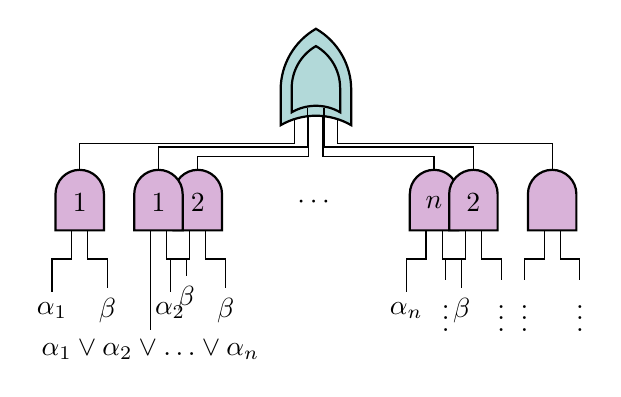
\begin{tikzpicture}[circuit logic US,every circuit symbol/.style={thick,point up}]
      \onslide<1-2>{
      \newOrNode{r}{0,0}{}{inputs=nnnn};
      \newAndNode{e1}{$(r)+(-3,-1.5)$}{1}{inputs=nn};
      \newAndNode{e2}{$(r)+(-1.5,-1.5)$}{2}{inputs=nn};
      \newAndNode{en}{$(r)+(1.5,-1.5)$}{$n$}{inputs=nn};
      \newAndNode{el}{$(r)+(3,-1.5)$}{}{inputs=nn};
      \node (ei) at ($(r)+(0,-1.5)$) {$\cdots$};
      \draw (r.input 1) -- ++(0,-0.3) -| (e1.east);
      \draw (r.input 2) -- ++(0,-0.5) -| (e2.east);
      \draw (r.input 3) -- ++(0,-0.5) -| (en.east);
      \draw (r.input 4) -- ++(0,-0.3) -| (el.east);
      \node (p1) at ($(e1.input 1)+(-0.25,-1.0)$) {$\alpha_1$};
      \node (s1) at ($(e1.input 2)+(0.25,-1.0)$) {$\beta$};
      \node (p2) at ($(e2.input 1)+(-0.25,-1.0)$) {$\alpha_2$};
      \node (s2) at ($(e2.input 2)+(0.25,-1.0)$) {$\beta$};
      \node (pn) at ($(en.input 1)+(-0.25,-1.0)$) {$\alpha_n$};
      \node (sn) at ($(en.input 2)+(0.25,-1.0)$) {$\beta$};
      \node (pl) at ($(el.input 1)+(-0.25,-1.0)$) {$\vdots$};
      \node (sl) at ($(el.input 2)+(0.25,-1.0)$) {$\vdots$};
      \draw (e1.input 1) -- ++(0,-0.35) -| (p1);
      \draw (e1.input 2) -- ++(0,-0.35) -| (s1);
      \draw (e2.input 1) -- ++(0,-0.35) -| (p2);
      \draw (e2.input 2) -- ++(0,-0.35) -| (s2);
      \draw (en.input 1) -- ++(0,-0.35) -| (pn);
      \draw (en.input 2) -- ++(0,-0.35) -| (sn);
      \draw (el.input 1) -- ++(0,-0.35) -| (pl);
      \draw (el.input 2) -- ++(0,-0.35) -| (sl);
      }\only<3>{
      \newOrNode{r}{0,0}{}{inputs=nn};
      \newAndNode{e1}{$(r)+(-2,-1.5)$}{1}{inputs=nn};
      \newAndNode{e2}{$(r)+(2,-1.5)$}{2}{inputs=nn};
      \draw (r.input 1) -- ++(0,-0.5) -| (e1.east);
      \draw (r.input 2) -- ++(0,-0.5) -| (e2.east);
      \node (p1) at ($(e1.input 1)+(0,-1.5)$) {$\alpha_1\vee\alpha_2\vee\ldots\vee\alpha_n$};
      \node (s1) at ($(e1.input 2)+(0.25,-0.85)$) {$\beta$};
      \node (p2) at ($(e2.input 1)+(-0.25,-1.0)$) {$\vdots$};
      \node (s2) at ($(e2.input 2)+(0.25,-1.0)$) {$\vdots$};
      \draw (e1.input 1) -- ++(0,-0.65) -| (p1);
      \draw (e1.input 2) -- ++(0,-0.35) -| (s1);
      \draw (e2.input 1) -- ++(0,-0.35) -| (p2);
      \draw (e2.input 2) -- ++(0,-0.35) -| (s2);
      }
    \end{tikzpicture}
  \end{center}
  \vskip 0.35cm
  \only<1>{We can generate $\sum_{k=1}^n\binom{n}{k}$ different circuits.}
  \only<2>{Uniformly sample a circuit from Pascal Triangle's $k$-th row.}
  \only<3>{But how to efficiently compute potentially complex disjunctions?}
\end{frame}

\begin{frame}[fragile]
  \frametitle{Binary Decision Diagrams (BDDs)}

  \begin{center}
    \begin{minipage}[b]{0.30\textwidth}
    \centering
    \resizebox{\textwidth}{!}{
    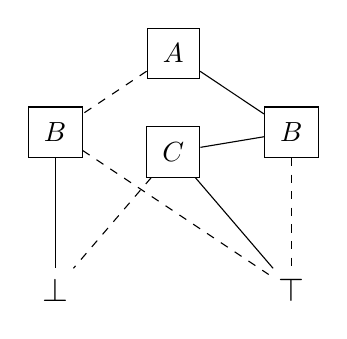
\begin{tikzpicture}
      \node[draw,inner sep=2mm] (a) at (0,0) {$A$};
      \node[draw,inner sep=2mm] (b1) at (-1.5, -1.0) {$B$};
      \node[draw,inner sep=2mm] (b2) at (1.5, -1.0) {$B$};
      \node[draw,inner sep=2mm] (c) at (0.0, -1.25) {$C$};
      \node (F) at (-1.5, -3.0) {\large$\bot$};
      \node (T) at (1.5, -3.0) {\large$\top$};
      \draw[dashed] (a) -- (b1);
      \draw (a) -- (b2);
      \draw[dashed] (b1) -- (T);
      \draw (b1) -- (F);
      \draw[dashed] (b2) -- (T);
      \draw (b2) -- (c);
      \draw[dashed] (c) -- (F);
      \draw (c) -- (T);
    \end{tikzpicture}
    }
  \end{minipage}
  ~
  \begin{minipage}[b]{0.65\textwidth}
    \centering
    \resizebox{\textwidth}{!}{
    \begin{tabular}{lll}
      \multicolumn{1}{l}{\bfseries Operation} & \multicolumn{1}{l}{\bfseries Description} &
      \multicolumn{1}{l}{\bfseries Complexity}\\
      \hline
      \textrm{\textproc{Reduce}} & canonical form of $\phi$ & $\bigo(n\cdot\log n)$\\
      \textrm{\textproc{Apply}} & $\phi_1\oplus\phi_2$ & $\bigo(n_1\cdot n_2)$\\
      \textrm{\textproc{Restrict}} & $\phi|_{x}$ & $\bigo(n\cdot\log n)$\\
      \textrm{\textproc{Forget}} & $\phi|_{x}\vee\phi|_{\neg x}$ & $\bigo(n^2)$
    \end{tabular}
    }
    \vspace{0.1cm}
  \end{minipage}
  \end{center}
  \vskip 0.5cm
  \begin{equation*}
    \phi(A,B,C)=(A\vee\neg B)\wedge(\neg B\vee C)
  \end{equation*}
\end{frame}

\section{Results}

\begin{frame}
  \frametitle{Likelihood}
  \centering\small
  \resizebox{\textwidth}{!}{
  \begin{tabular}{cr|ccc|cccc}
    \hline
    \multicolumn{1}{c}{\bfseries Data} & \multicolumn{1}{c}{\bfseries \#vars} &
    \multicolumn{1}{c}{\bfseries Worst} & \multicolumn{1}{c}{\bfseries Best} &
    \multicolumn{1}{c}{\bfseries Average} & \multicolumn{1}{c}{\bfseries LSPN-Opt} &
    \multicolumn{1}{c}{\bfseries LSPN-CV} & \multicolumn{1}{c}{\bfseries CLT} &
    \multicolumn{1}{c}{\bfseries CNet}\\
    \hline
    1 & 10 & -449.89 & \textbf{-413.51} & \underline{-415.60} & -422.37 & -444.62 & -456.49 & -585.23\\
    2 & 15 & -745.20 & \textbf{-693.51} & -695.82 & \underline{-695.09} & -739.49 & -803.41 & -1070.29\\
    3 & 20 & -1024.01 & \underline{-969.51} & -971.80 & \textbf{-959.03} & -1003.93 & -1075.31 & -1855.05\\
    4 & 25 & -1268.82 & \underline{-1208.22} & -1210.27 & \textbf{-1185.28} & -1254.47 & -1290.94 & -2033.58\\
    5 & 30 & -1548.92 & \textbf{-1440.27} & -1442.58 & \underline{-1441.90} & -1543.35 & -1535.54 & -2048.16\\
    6 & 100 & -5169.14 & \underline{-4995.53} & -4997.83 & \textbf{-4958.06} & -5232.04 & -5712.73 & -10326.73\\
    7 & 100 & -5329.17 & \underline{-5153.51} & -5155.82 & \textbf{-4900.65} & -5206.54 & -5710.64 & -9948.88\\
    8 & 14 & -472.15 & \textbf{-423.32} & \underline{-425.62} & -490.21 & -506.62 & -486.06 & -601.31
  \end{tabular}
  }
  \vskip 0.25cm
  \footnotesize
  \resizebox{\textwidth}{!}{
  \begin{tabular}{c|l}
    \hline
    \multicolumn{1}{c}{\bfseries Data} & \multicolumn{1}{l}{\bfseries Logic formula}\\
    \hline
    1 & $\phi_1=(X_1\wedge X_3)\vee(X_4\wedge\neg X_2)\vee(X_5\wedge\neg X_{10})$\\
    2 & $\phi_2=(X_1\wedge X_3)\vee(X_4\wedge\neg X_2)\vee(X_5\wedge\neg X_{10})\vee(X_{12}\wedge\neg
    X_{13}\wedge X_{15}\wedge\neg X_{14})$\\
    3 & $\phi_3=(X_1\wedge X_3)\vee(X_4\wedge\neg X_2)\vee(X_5\wedge\neg X_{10})\vee(X_{12}\wedge\neg
    X_{13}\wedge X_{15}\wedge\neg X_{14})$\\
    4 & $\phi_4=(X_1\wedge X_3)\vee(X_4\wedge\neg X_2)\vee(X_5\wedge\neg X_{10})\vee(X_{12}\wedge\neg
    X_{13}\wedge X_{15}\wedge\neg X_{14})$\\
    5 & $\phi_5=(X_2\vee X_{30})\wedge(\neg X_{15}\vee\neg X_{10})\wedge(\neg X_{25}\vee X_5\vee
    X_{15}\vee\neg X_1)\wedge(X_1\vee X_{15}\vee\neg X_{30})$\\
    6 & $\phi_6=(X_{10}\vee X_{30})\wedge(\neg X_1\vee X_5)\wedge(\neg X_{10}\vee X_{14}\vee
    X_{23})\wedge(X_2\vee\neg X_{27}\vee X_{35})\wedge(X_{98}\vee\neg X_{78}\vee\neg X_{27}\vee
    X_8)$\\
    7 & $\phi_7=\top$\\
    8 & $\phi_8=d_0\vee d_1\vee d_2\vee d_3\vee d_4\vee d_5\vee d_6\vee d_7\vee d_8\vee d_9$\\
  \end{tabular}
  }
\end{frame}

\begin{frame}
  \begin{centering}
  \begin{beamercolorbox}[sep=12pt,center]{part title}
  \usebeamerfont{section title}Thank You!\\\vskip 0.5cm Questions?\par
  \end{beamercolorbox}
  \end{centering}
\end{frame}

\section{References}

\begin{frame}[t,allowframebreaks]
  \frametitle{References}
  \printbibliography[heading=none]
\end{frame}

\end{document}
